\documentclass[11pt, oneside]{book}

\usepackage{pdfpages}
\usepackage{xepersian}
\settextfont{Yas}
\setdigitfont{Yas}

\begin{document}
\frontmatter
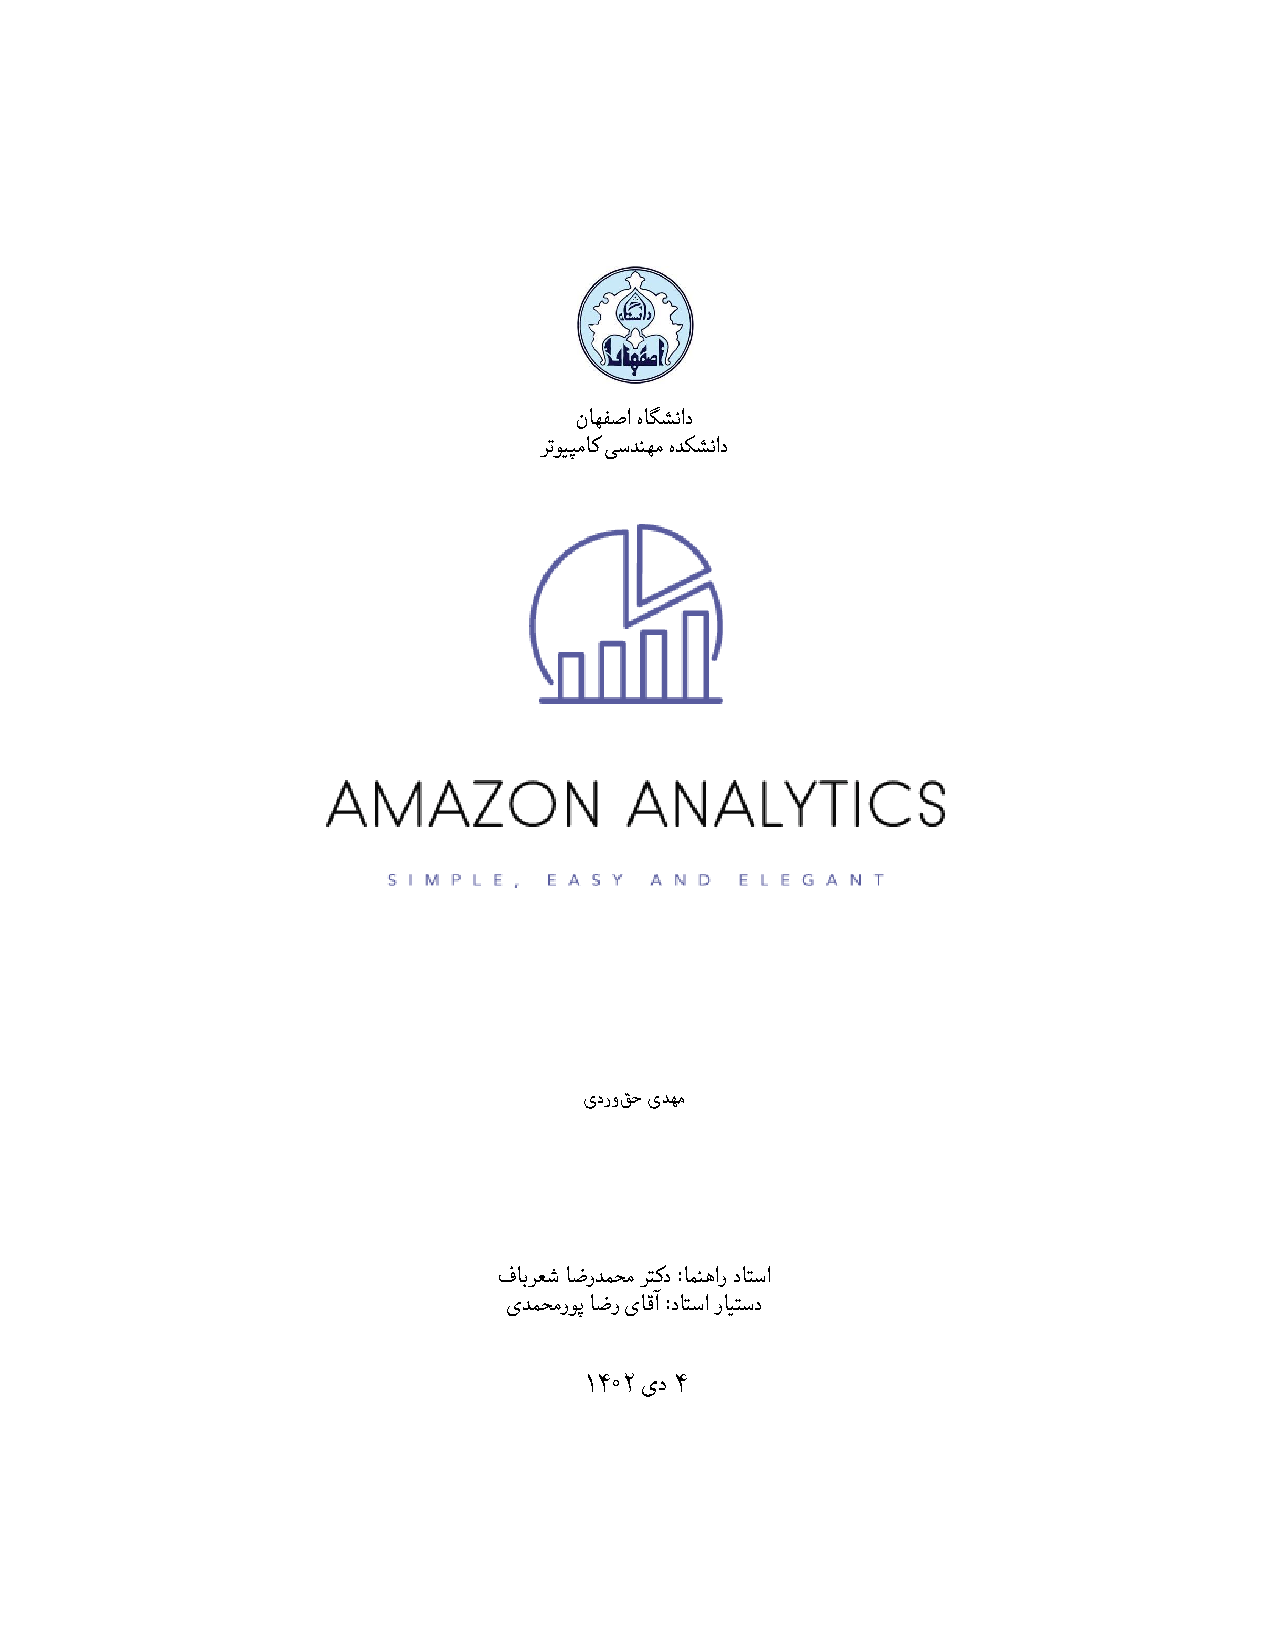
\includepdf{../titlepage/atitle}
\tableofcontents
\mainmatter

\chapter{توضیحات نسخه دمو}
در این فصل به بررسی آنچه که از پروژه‌ی 
\lr{Amazon Analytics}
به صورت دمو پیاده‌سازی می‌شود، پرداخته می‌شود. آنچه که لازم به ذکر است این‌ست که، تمامی مطالعات صورت گرفته برای پروژه‌ی
\lr{Amazon Analytics}
انجام شده، بر اساس پیاده‌سازی از صفر بوده، و همچنین با توجه به فاز سوم پروژه، نیازمند حداقل ۱۳ ماه برای پیاده‌سازی است. به همین جهت، نسخه‌ی دمو تنها قسمت کوچکی از اصل پروژه خواهد بود.

\section{قسمت‌های نسخه‌ی دمو}
نسخه‌ی دمو قرار است که بر اساس یک سری داده‌ی ذخیره شده، خروجی‌های مختلفی که در پروژه به آنها پرداخته شده بود، را نشان بدهد. در این بخش قسمت‌های مختلف را نام برده و به بررسی خروجی آنها می‌پردازیم.

\subsection{بخش کاربران}
\subsection{بخش \lr{Stock}}
\subsection{بخش \lr{Site}}
\subsection{بخش \lr{Shipment}}

\end{document}